% -*- coding: UTF-8 -*-
% vim: autoindent expandtab tabstop=4 sw=4 sts=4 filetype=tex
% vim: spelllang=de spell
% chktex-file 27 - disable warning about missing include files

\chapter{Prototyp}
\label{chap:prototype}

Um das Sphere Tracing Verfahren nicht nur theoretisch zu betrachten,
wurde im Rahmen dieser Projektarbeit ein Prototyp erstellt. Dieser
wurde in C++ Version 11 und OpenGL umgesetzt und basiert auf der
GLFW-Bibliothek. Um allfällige OpenGL-Erweiterungen (Extensions) nicht
selbst verwalten zu müssen, wird GLEW eingesetzt. Als Buildsystem kommt
CMake, als Compiler GCC zum Einsatz. Um automatisch Shader erkennen und
laden zu können (Dateien mit Dateiendung~.vs bzw.~.fs), werden die
Bibliotheken ``system'',  ``filesystem'' sowie ``regex'' der
Boost-Bibliothek benützt.

% -*- coding: UTF-8 -*-
% vim: autoindent expandtab tabstop=4 sw=4 sts=4 filetype=tex
% vim: spelllang=de spell
% chktex-file 27 - disable warning about missing include files

\section{Komponenten}
\label{sec:main-components}

Ausgehend von den Anforderungen (\ref{sec:requirements}) können einzelne
Komponenten der Applikation abgeleitet werden. Einzelne Teile davon wurden
schon durch die Vision (\ref{sec:vision}) definiert beziehungsweise aus dieser
gewonnen.

Dieser Prozess entspricht nicht direkt dem Vorgehen
gemäss~\cite{larman_applying_2004} beziehungsweise dem UP, der Autor dieser
Projektarbeit ist jedoch der Ansicht, dass dieser Abschnitt eine Brücke
zwischen Anforderungen und der (Software-) Modellierung bildet. Zudem bietet
dieser Abschnitt eine relativ bildliche Beschreibung, was dem Verständnis des
Gesamtkonzeptes sicher zuträglich ist. Am ehesten entspricht dieser Abschnitt
den Komponenten-Diagrammen in~\cite[S. 653 bis 654]{larman_applying_2004}.

Die Applikation besteht aus zwei Applikationen: Einem \textit{Player},
welcher dem Abspielen von Echtzeit-Animationen dient, sowie einem \textit{Editor},
welcher der Erstellung und Verwaltung von Echtzeit-Animationen dient.

\subsection{Player}
\label{subsec:main-components:player}

Der \textit{Player} liest die vom \textit{Editor} exportierten
Echtzeit-Animationen. Er bietet vor dem Abspielen die Auswahl der Auflösung,
des Seitenverhältnisses, Antialiasing und ob die Animation im Vollbild-Modus
abgespielt werden soll.

\subsection{Editor}
\label{subsec:main-components:editor}

Der \textit{Editor} erlaubt das Erstellen und Bearbeiten von
Echtzeit-Animationen. Diese können schliesslich inklusive den
dazugehörigen Dateien, wie zum Beispiel Bitmaps oder Modellen, exportiert
werden.

\begin{figure}[h]
    \centering
    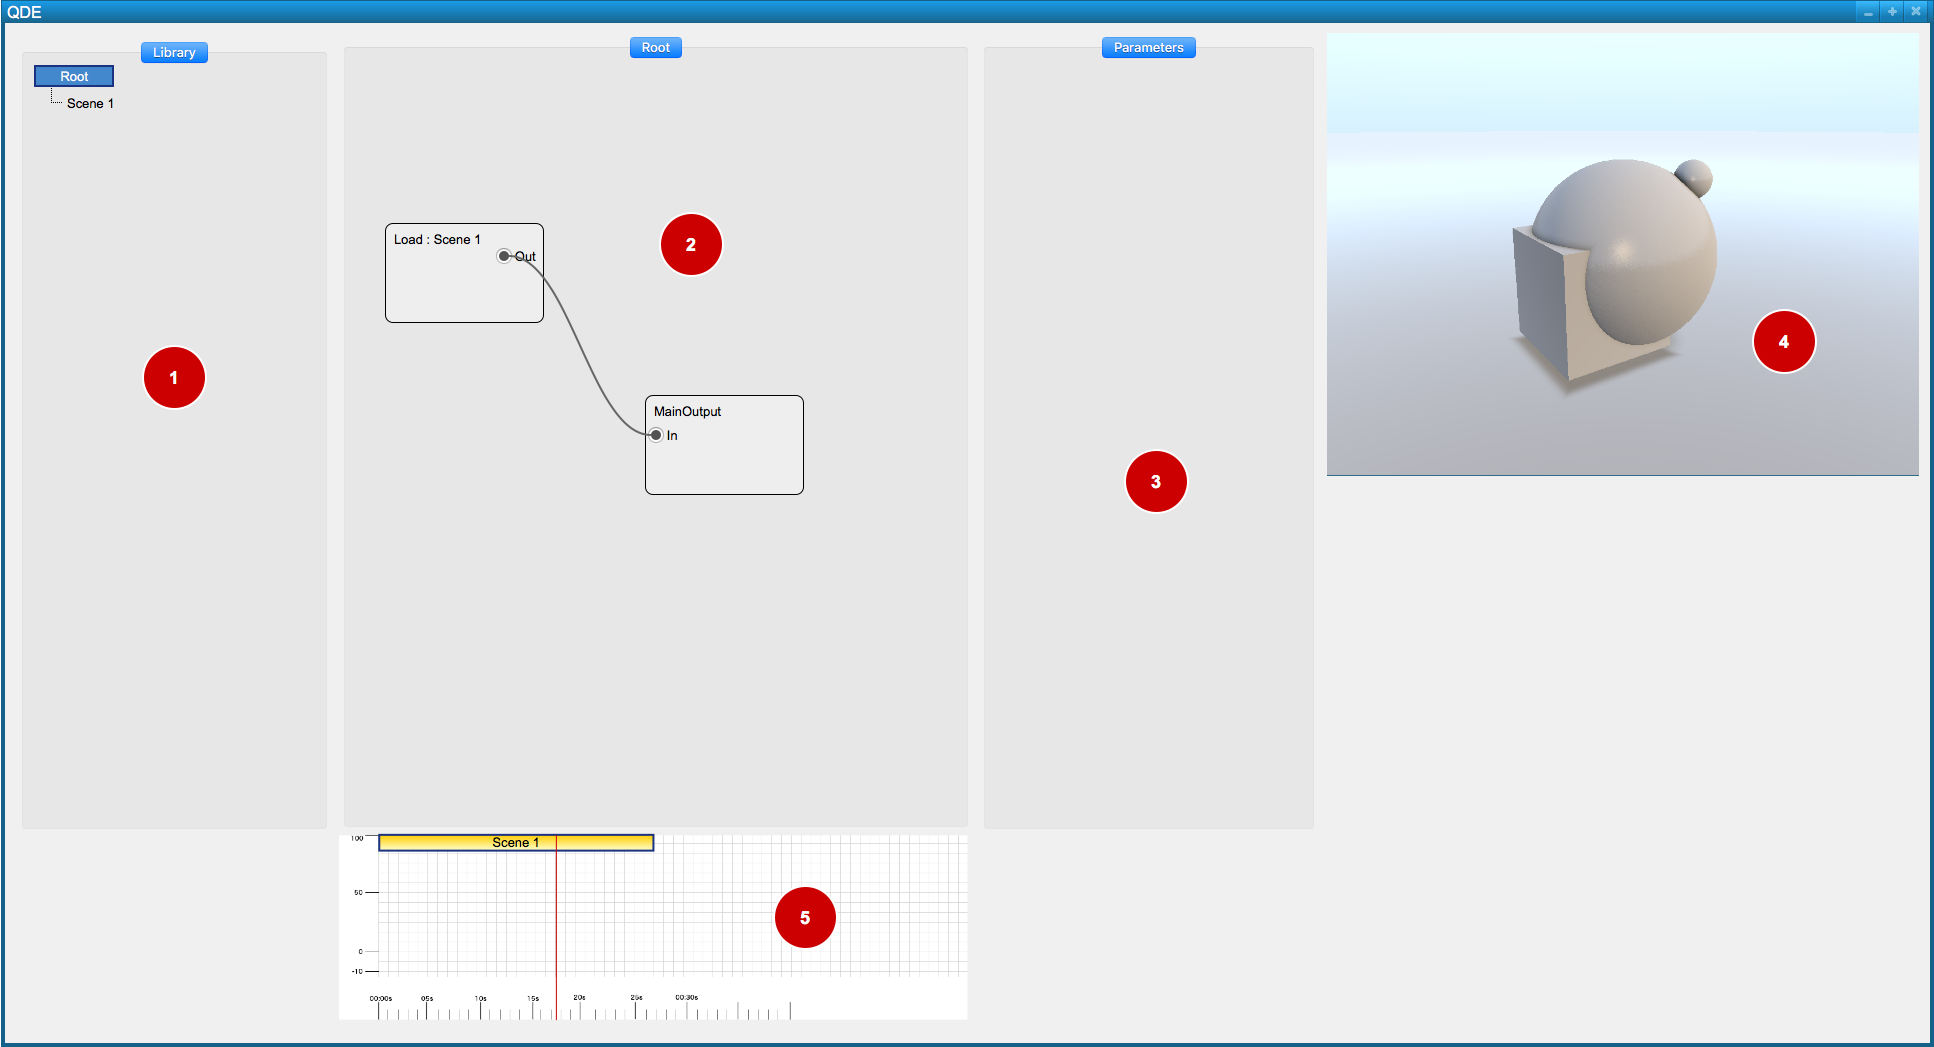
\includegraphics[width=0.9\textwidth]{img/editor_components.png}
    \caption{Einzelne Komponenten des Editors
        \protect\footnotemark}\label{fig:main-components:editor:editor-components}
\end{figure}
\footnotetext{Eigene Darstellung mittels Pencil.}

Abbildung~\ref{fig:main-components:editor:editor-components} zeigt die
einzelnen Komponenten des Editors. Nachfolgend findet sich eine Beschreibung
dieser.

\subsubsection{Bibliothek}
\label{ssubsec:main-components:editor:library}

Das Element~\img{img/editor_component_1.png} in
Abbildung~\ref{fig:main-components:editor:editor-components} zeigt die (Szenen-)
Bibliothek. Diese beinhaltet alle Szenen einer Echtzeit-Animation. Es können
neue Szenen angelegt und auch bestehende Szenen gelöscht werden. Wird ein neues
Projekt erstellt, so verfügt dieses immer über die ``Root''-Szene. Diese
beinhaltet den Haupt-Ausgabeknoten des Graphen
(\ref{ssubsec:main-components:editor:graph}), welcher schliesslich zum
Abspielen evaluiert wird, und kann nicht gelöscht werden. Wird eine Szene mit
der Maus angewählt, so wird deren Inhalt im Graphen
(\ref{ssubsec:main-components:editor:graph}) dargestellt.

\subsubsection{Graph}
\label{ssubsec:main-components:editor:graph}

Das Element~\img{img/editor_component_2.png} in
Abbildung~\ref{fig:main-components:editor:editor-components} zeigt den Graphen
einer Szene. Dieser beinhaltet sämtliche Knoten einer Szene. Mittels
Kontextmenü können neue Knoten eingefügt und bestehende Knoten gelöscht werden.
Wird ein Knoten angewählt, so wird dieser einerseits im
Rendering-Ansichtsfenster (\ref{ssubsec:main-components:editor:rendering})
dargestellt, andererseits werden dessen Eigenschaften im Parameter-Fenster
(\ref{ssubsec:main-components:editor:parameters}) angezeigt.

Folgende Typen von Knoten sind geplant:
\begin{itemize}
    \item{Scene}
    \item{TimelineClip}
    \item{Model}
    \item{Camera}
    \item{Light}
    \item{Material}
    \item{Operator}
    \item{Effect}
\end{itemize}

\subsubsection{Parameter}
\label{ssubsec:main-components:editor:parameters}

Das Element~\img{img/editor_component_3.png} in
Abbildung~\ref{fig:main-components:editor:editor-components} zeigt die Parameter
des aktuell gewählten Knoten im Graphen
(\ref{ssubsec:main-components:editor:graph}). Neben jedem Parameter befindet
sich eine Schaltfläche zum Setzen von Schlüsselbildern (Keyframes) in der
Zeitachse (Timeline,~\ref{ssubsec:main-components:editor:timeline}). Wird die
Schaltfläche betätigt, so wird bei dem aktuell ausgewählten Zeitpunkt der
Zeitachse ein Schlüsselbild gesetzt.

\subsubsection{Rendering}
\label{ssubsec:main-components:editor:rendering}

Das Element~\img{img/editor_component_4.png} in
Abbildung~\ref{fig:main-components:editor:editor-components} zeigt das
Rendering-Ansichtsfenster. Dieses stellt den Inhalt des aktuell gewählten
Knotens dar. Die Art des Knotens ist dabei nicht beschränkt, es kann dies eine
Szene, aber zum Beispiel auch ein einzelnes Modell sein. Es wird immer der
gesamte vorhergehende (Teil-) Baum des Knotens evaluiert.

\subsubsection{Zeitachse}
\label{ssubsec:main-components:editor:timeline}

Die Zeitachse wird mit~\img{img/editor_component_5.png} in
Abbildung~\ref{fig:main-components:editor:editor-scene1} dargestellt.  Sie
bildet das zeitliche Geschehen einer Echtzeit-Animation ab. Alle Knoten vom Typ
Timeline-Clip werden am oberen Rand des Fensters in deren zeitlicher
Reihenfolge abgebildet. Wird im Graph
(\ref{ssubsec:main-components:editor:graph}) ein Knoten mit animierten
Parametern (\ref{ssubsec:main-components:editor:parameters}) angewählt, so sind
diese ersichtlich. Vertikal wird der Wertebereich, horizontal die Zeitachse in
Sekunden dargestellt. Ein vertikal verlaufender, roter Marker zeigt die aktuelle
zeitliche Position der Echtzeit-Animation an.

Die untenstehende Abbildung~\ref{fig:main-components:editor:editor-scene1} zeigt ein Beispiel, wie eine typische Szene
mit animierten Parametern aussehen könnte.

\begin{figure}[H]
    \centering
    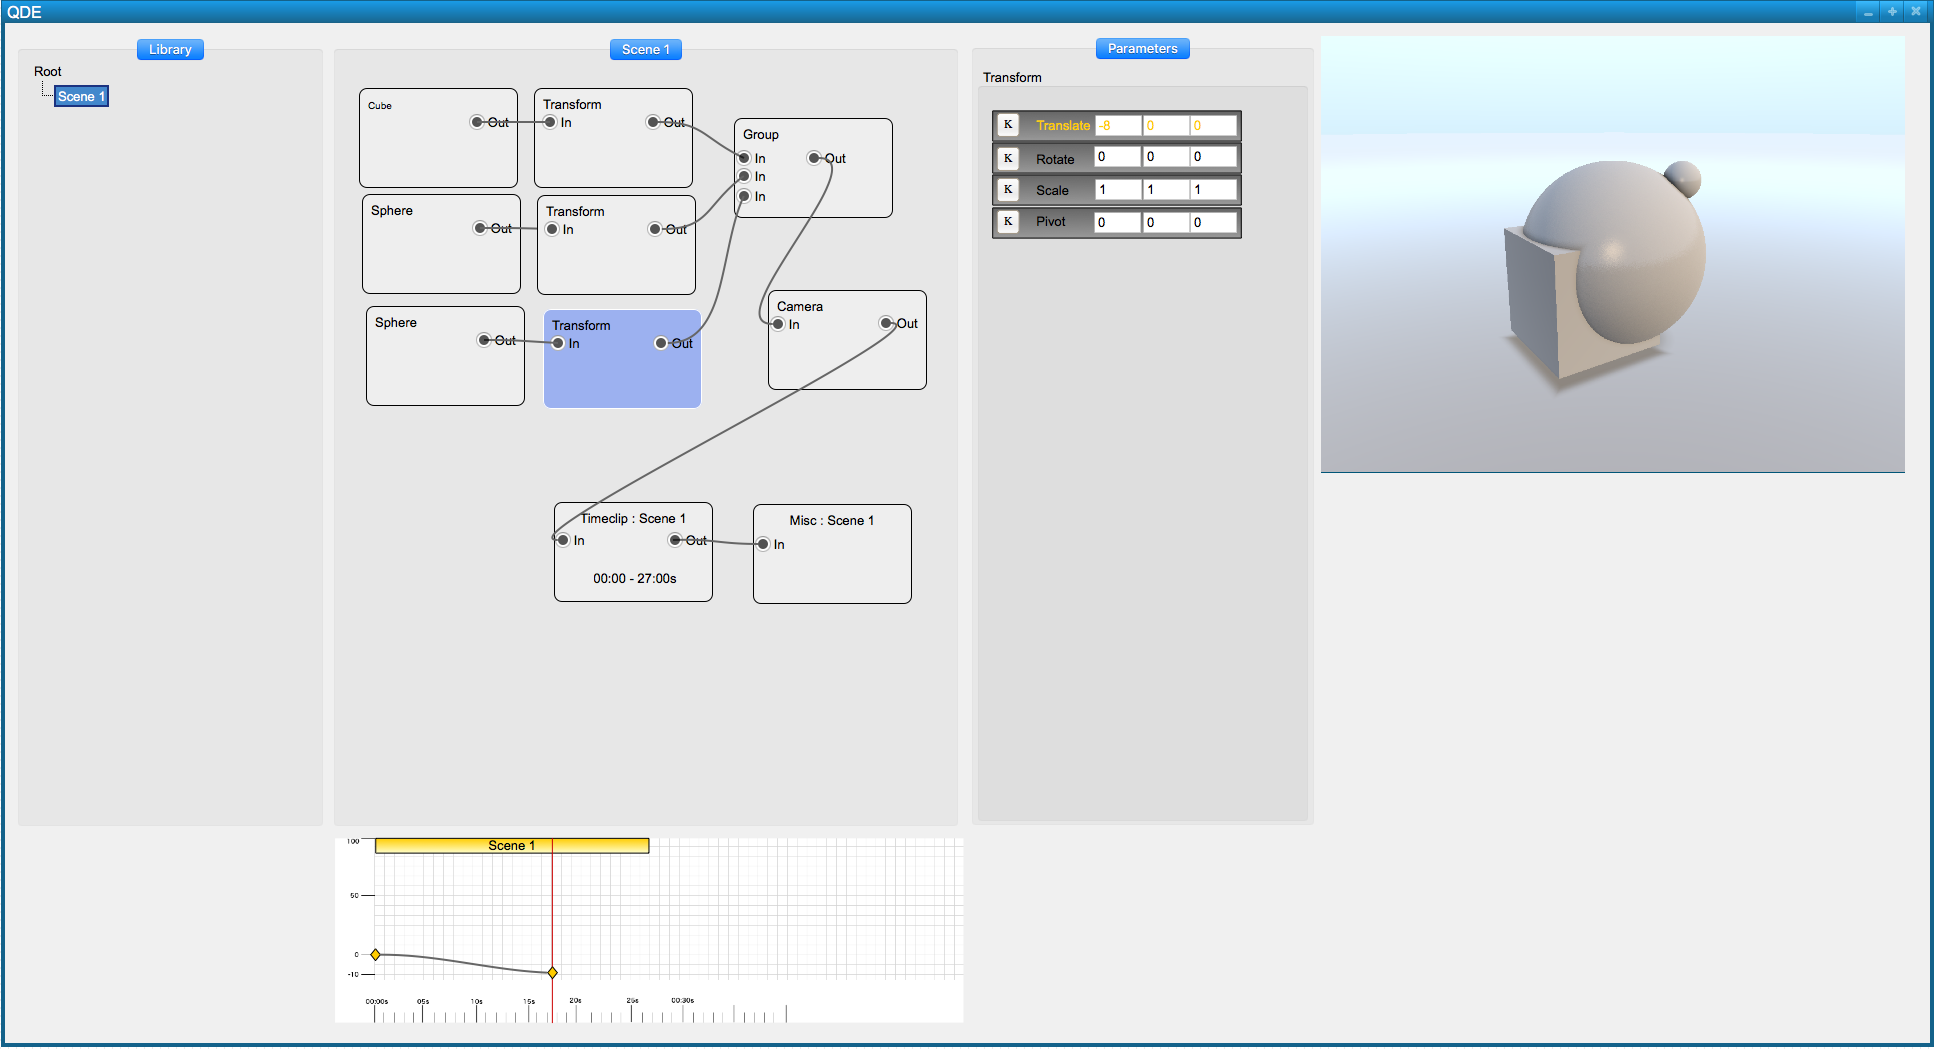
\includegraphics[width=0.9\textwidth]{img/editor_scene1.png}
    \caption{Beispiel-Szene innerhalb des Editors
        \protect\footnotemark}\label{fig:main-components:editor:editor-scene1}
\end{figure}
\footnotetext{Eigene Darstellung mittels Pencil.}

% -*- coding: UTF-8 -*-
% vim: autoindent expandtab tabstop=4 sw=4 sts=4 filetype=tex
% vim: spelllang=de spell
% chktex-file 27 - disable warning about missing include files

\section{Architektur}
\label{sec:architecture}

Die Architektur des~\hyperref[chap:prototype]{Prototypen} wurde bewusst einfach gehalten und ist
in~\autoref{fig:prototype_architecture} ersichtlich.

% \begin{figure}[H]
%     \centering
%     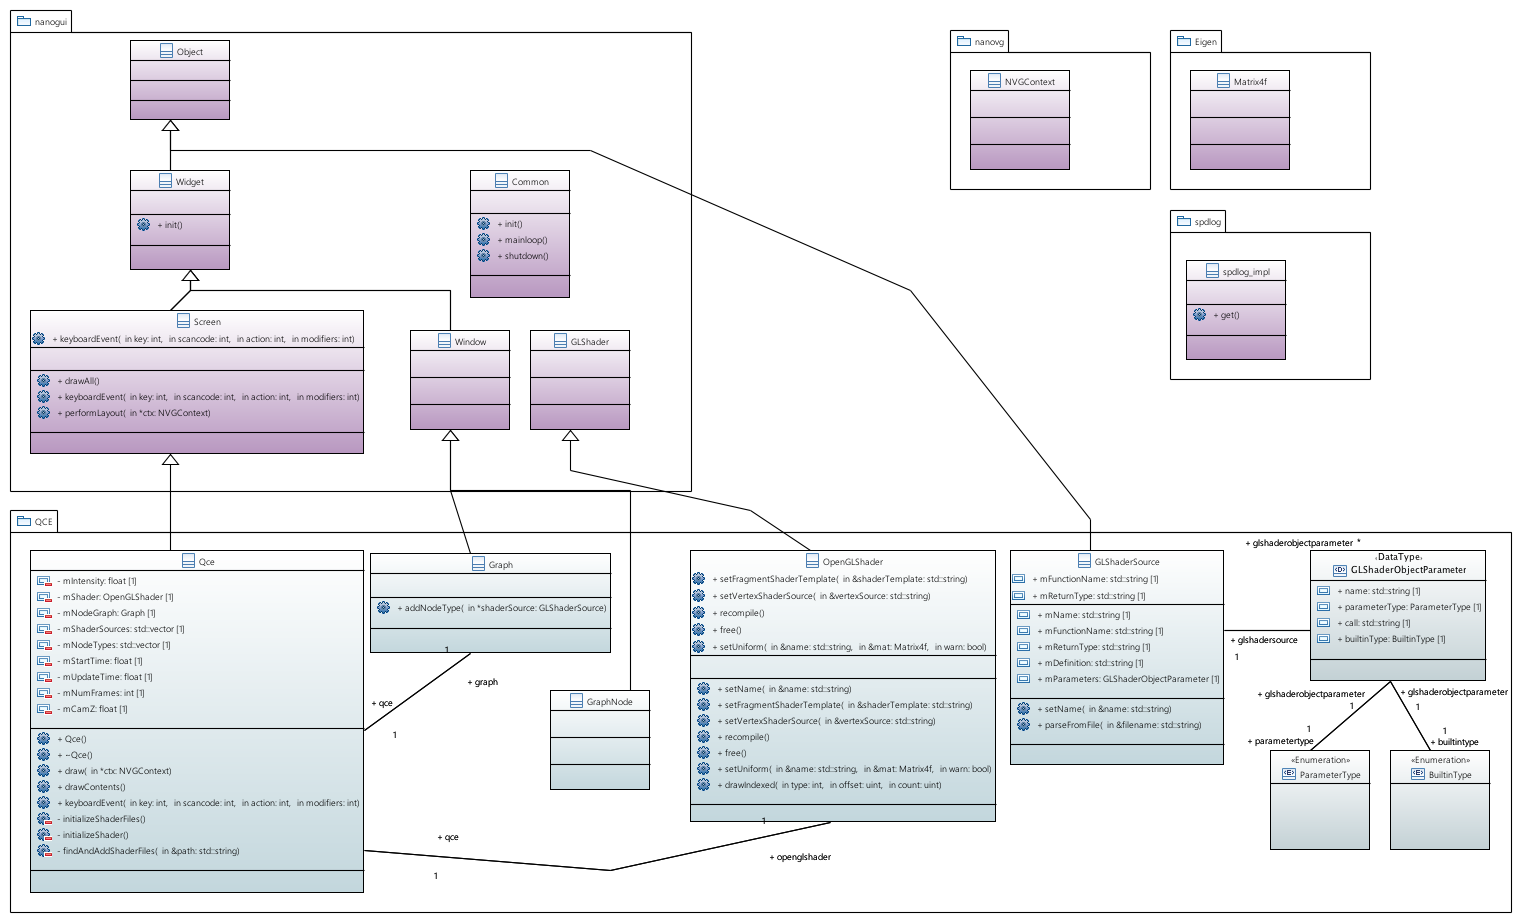
\includegraphics[width=0.8\textwidth]{img/prototype_class_diagram.pdf}
%     \caption{Architektur des~\hyperref[chap:prototype]{Prototypen}\protect\footnotemark}\label{fig:prototype_architecture}
% \end{figure}
\footnotetext{Eigene Darstellung mittels yEd.}

\subsection{Programmablauf}
\label{subsec:program_sequence}

Wie aus~\autoref{fig:prototype_architecture} ersichtlich, besteht die
Applikation hauptsächlich aus der Hauptfunktion \textit{``Main''}. Diese
benützt GLEW um OpenGL zu initialisieren. Mittels GLFW erstellt sie ein
Fenster sowie einen OpenGL-Kontext. Danach wird eine Instanz der Klasse
\textit{ShaderFactory} erstellt, welche ihrerseits alle verfügbaren
GLSL-Shader aus einem gegebenen Verzeichnis lädt. Bei diesem~\hyperref[chap:prototype]{Prototypen}
kommt jedoch nur ein einziger Shader zum Einsatz. Er bestehent aus einem
\textit{Vertex}- und einem \textit{Fragment}-Teil.

Die Applikation läuft danach in einer Endlosschleife, hört dabei aber
auf Events in Form von Keyboard-Eingaben. Dadurch kann die Applikation
jederzeit mit der Abbruch-Taste (ESC, Escape) beendet werden.

Die hauptsächliche Aufgabe der Applikation besteht aus dem Laden und
Ausführen eines Vertex- sowie Fragment-Shaders im Rendering-Teil.  Dazu
wird via OpenGL ein Rechteck über die verfügbare Fläche des Fensters
ausgegeben.  Der Vertex-Shader adressiert schliesslich das von OpenGL
gezeichnete Rechteck.  Das eigentliche Rendering von impliziten
Oberflächen geschieht schliesslich im Fragment-Shader. Dies ist in der
untenstehenden~\autoref{fig:prototype_shaders} verdeutlicht.

% \begin{figure}[H]
%     \centering
%     \includegraphics[width=0.8\textwidth]{img/prototype_shaders.pdf}
%     \caption{Bildliche Darstellung der Funktionsweise von Vertex- und
%         Fragment-Shader der Applikation\protect\footnotemark}\label{fig:prototype_shaders}
% \end{figure}
\footnotetext{Eigene Darstellung mittels yEd.}

% -*- coding: UTF-8 -*-
% vim: autoindent expandtab tabstop=4 sw=4 sts=4 filetype=tex
% vim: spelllang=de spell
% chktex-file 27 - disable warning about missing include files

\section{Umsetzung}
\label{sec:realization}

Nachfolgend werden die
gemäss~\autoref{sec:description_implicit_surfaces} umgesetzten Konzepte
genauer beschrieben. Es handelt sich dabei um Ausschnitte des
umgesetzten Fragment-Shaders.

Das eigentliche Sphere Tracing geschieht in der Funktion
\textit{castRay}.  Diese hat als Parameter den Ursprung eines Strahles
(\textit{vec3 rayOrigin}), die Richtung eines Strahles (\textit{vec3
    rayDirection}), die maximale Distanz (\textit{float maxDistance}),
welche berechnet werden soll, die Präzision (\textit{float precision})
sowie die Anzahl Durchgänge (\textit{int steps}).

Ein Vergleich der letzten drei Parameter --- die maximale Distanz, die
Präzision sowie die Anzahl Durchgänge --- findet sich in den
Tabellen~\ref{table:sphere_tracing_distance},~\ref{table:sphere_tracing_precision}
und~\ref{table:sphere_tracing_steps}.

Maschinell bedingt kommen bei den Berechnungen Fliesskommazahlen zum
Einsatz, da die Resultate möglichst genau sein sollen. Aufgrund der
endlichen Mantisse bei der Darstellung von Fliesskommazahlen lassen sich
diese auf einem Computer jedoch nicht beliebig genau darstellen und
damit berechnen. Rundung und damit verbundene Rundungsfehler sind
unvermeidlich.  Um dennoch eine gute Annäherung an Null-Werte zu
erhalten, wird ein Parameter ($\varepsilon$) zur Steuerung der minimalen
Distanz zu einer Oberfläche verwendet. Dieser kommt bei den
Funktionen~\textit{render}, \textit{castRay} sowie \textit{calcShadows}
in Form der Variablen \textit{minimalDistance} bzw.  \textit{precision}
zum Einsatz.

\begin{minipage}{\linewidth}
\begin{lstlisting}[language=GLSL,caption={Umsetzung des Sphere Tracings in
        GLSL.},label={alg:glsl_sphere_tracing},captionpos=b,emph={castRay}]
// Casts a ray from given origin i given direction. Stops at given
// maximal distance and after given amount of steps. Maintains given
// precision.
vec2 castRay(in vec3 rayOrigin, in vec3 rayDirection, in float maxDistance, in float precision, in int steps)
{
    float latest    = precision * 2.0;
    float distance  = 0.0;
    float type      = -1.0;
    vec2  res       = vec2(-1.0, -1.0);

    for(int i = 0; i < steps; i++) {
        if (abs(latest) < precision || distance > maxDistance) {
            continue;
        }

        vec2 result = scene(rayOrigin + rayDirection * distance);

        latest     = result.x;
        type       = result.y;
        distance  += latest;
    }

    if (distance < maxDistance) {
        res = vec2(distance, type);
    }

    return res;
}
\end{lstlisting}
\end{minipage}

\begin{table}[H]
    \centering
    \caption{Vergleich des Distanz-Parameters anhand einer Beispielszene.}\label{table:sphere_tracing_distance}
    \begin{tabular}{p{0.3\textwidth}p{0.3\textwidth}p{0.3\textwidth}}
        \toprule
            \textbf{Distanz: \textit{100.0}} &
            \textbf{Distanz: \textit{9.0}}   &
            \textbf{Distanz: \textit{6.3}}   \\
        \cmidrule(r){1-1}\cmidrule(lr){2-2}\cmidrule(l){3-3}
            \includegraphics[width=0.3\textwidth]{img/sphere_tracing_distance_full.pdf}
            \newline
            Alle in der Szene definierten Objekte sind sichtbar. &
            \includegraphics[width=0.3\textwidth]{img/sphere_tracing_distance_less.pdf} \newline
            Es ist nur noch das zum Betrachter näher liegende Objekt sichtbar. &
            \includegraphics[width=0.3\textwidth]{img/sphere_tracing_distance_min.pdf} \newline
            Es ist nur noch das zum Betrachter näher liegende Objekt
            sichtbar, jedoch nicht mehr vollständig. \\
        \bottomrule
    \end{tabular}
\end{table}

\begin{table}[H]
    \centering
    \caption{Vergleich des Präzisions-Parameters anhand einer Beispielszene.}\label{table:sphere_tracing_precision}
    \begin{tabular}{p{0.3\textwidth}p{0.3\textwidth}p{0.3\textwidth}}
        \toprule
            \textbf{Präzision: \textit{0.00001}} &
            \textbf{Präzision: \textit{0.1}}     &
            \textbf{Präzision: \textit{1.0}}     \\
        \cmidrule(r){1-1}\cmidrule(lr){2-2}\cmidrule(l){3-3}
            \includegraphics[width=0.3\textwidth]{img/sphere_tracing_precision_full.pdf} \newline
            Die Kugel weist keinerlei sichtbare Abstufungen auf. &
            \includegraphics[width=0.3\textwidth]{img/sphere_tracing_precision_min.pdf} \newline
            Die Kugel weist am unteren linken Rand sichtbare Farbabstufungen auf. &
            \includegraphics[width=0.3\textwidth]{img/sphere_tracing_precision_pos.pdf} \newline
            Die Kugel wird nicht mehr korrekt dargestellt. \\
        \bottomrule
    \end{tabular}
\end{table}

\begin{table}[H]
    \centering
    \caption{Vergleich des Parameters zur Bestimmung der Anzahl der
        Durchgänge anhand einer Beispielszene.}\label{table:sphere_tracing_steps}
    \begin{tabular}{p{0.3\textwidth}p{0.3\textwidth}p{0.3\textwidth}}
        \toprule
            \textbf{Anzahl Schritte: \textit{100}} &
            \textbf{Anzahl Schritte: \textit{10}}  &
            \textbf{Anzahl Schritte: \textit{5}}   \\
        \cmidrule(r){1-1}\cmidrule(lr){2-2}\cmidrule(l){3-3}
            \includegraphics[width=0.3\textwidth]{img/sphere_tracing_steps_full.pdf} \newline
            Alle in der Szene definierten Objekte sind korrekt sichtbar. &
            \includegraphics[width=0.3\textwidth]{img/sphere_tracing_steps_less.pdf} \newline
            Die Grenze zwischen den in der Szene definierten Objekten
            ist bereits nicht mehr eindeutig. &
            \includegraphics[width=0.3\textwidth]{img/sphere_tracing_steps_min.pdf} \newline
            Die Szene ist als solche nicht mehr erkennbar, es erfolgt
            keine klare Trennung zwischen den einzelnen Objekten.  \\
        \bottomrule
    \end{tabular}
\end{table}

Von den unter~\autoref{subsec:implicit_surfaces_ops} beschriebenen
Operationen wurden die Operationen \textit{Vereinigung}, \textit{Subtraktion} sowie
\textit{Intersektion} umgesetzt.

\begin{minipage}{\linewidth}
\begin{lstlisting}[language=GLSL,caption={Umsetzung der Operationen
        \textit{Vereinigung}, \textit{Subtraktion} sowie
        \textit{Intersektion} für implizite Oberflächen in
        GLSL.},label={alg:glsl_ops},captionpos=b,emph={subtract,merge,intersect}]
// Returns the signed distance for a substraction of given signed
// distance a to signed distance b.
float subtract(float a, float b)
{
    return max(-b, a);
}

// Returns the signed distance for a merge of given signed
// distance a and signed distance b.
vec2 merge(vec2 a, vec2 b)
{
    return min(a, b);
}

// Returns the signed distance for a intersection  of given signed
// distance a and signed distance b.
float intersect(float a, float b)
{
    return (a > b) ? a : b;
}
\end{lstlisting}
\end{minipage}

Von den unter~\autoref{subsec:implicit_surfaces_primitives} beschriebenen
Primitiven wurden die Primitiven \textit{Ebene} sowie \textit{Kugel} umgesetzt.

\begin{minipage}{\linewidth}
\begin{lstlisting}[language=GLSL,caption={Umsetzung der Primitiven
        \textit{Ebene} und \textit{Kugel} in Form von impliziten
        Oberflächen in
        GLSL.},label={alg:glsl_primitives},captionpos=b,emph={plane,sphere,box}]
// Returns the signed distance to a plane for the given position.
float plane(vec3 position)
{
    return position.y;
}

// Returns the signed distance to a sphere with given radius for the
// given position.
float sphere(vec3 position, float radius)
{
    return length(position) - radius;
}

// Returns the signed distance to a box with given dimension for the
// given position.
float box(vec3 position, vec3 dimension)
{
    position = abs(position) - dimension;
    return max(max(position.x, position.y), position.z);
}
\end{lstlisting}
\end{minipage}

Verwendete Parameter sind jeweils die (gewünschte) Position des Objektes
(\textit{vec3 position}) sowie der Radius bzw.\ die Dimension
(\textit{float radius} bzw. \textit{vec3 dimension}).

Als Beleuchtungsmodell wurde das
unter~\autoref{sec:rendering_implicit_surfaces} beschriebene
Phong-Beleuchtungsmodell umgesetzt.

\begin{minipage}{\linewidth}
\begin{lstlisting}[language=GLSL,caption={Umsetzung des
        Phong-Beleuchtungsmodelles in
        GLSL.},label={alg:glsl_lighting},captionpos=b,emph={calcLighting}]
// Calculates the lighting for the given position, normal and direction,
// the given light (position and color) respecting the 'material'.
//
// This is mainly applying the phong lighting model inlcuding shadows.
//
// Returns the calculated color as three-dimensional vector.
vec3 calcLighting(vec3 normal, vec3 rayDirection) {

    vec3 lightDirection     = normalize(vec3(0.0, 4.0, 5.0));

     float kDirectLight      = 0.1;
     float shadows           = calcShadows(position, lightDirection);
     vec3  direct            = vec3(kDirectLight * shadows);

    vec3 ambientColor       = vec3(0.05, 0.15, 0.2);
    float kAmbient          = clamp(0.5 + 0.5 * normal.y, 0.0, 1.0);
    vec3 ambient            = kAmbient * ambientColor;

    vec3 diffuseColor       = vec3(0.2, 0.6, 0.8);
    float kDiffuse          = clamp(dot(lightDirection, normal), 0.0, 1.0);
    vec3 diffuse            = kDiffuse * diffuseColor;

    vec3 specularColor      = vec3(1.0);
    float kSpecularExponent = 24.0;
    vec3 h                  = normalize(-rayDirection + lightDirection);
    float nFacing           = clamp(dot(lightDirection, normal), 0.0, 1.0);
    float kSpecular         = pow(clamp(dot(h, normal), 0.0, 1.0), kSpecularExponent);
    vec3 specular           = nFacing * kSpecular * specularColor;

     vec3 light              = ambient + diffuse + specular + direct;
     vec3 color              = material * light;
 
     return color;
}
\end{lstlisting}
\end{minipage}

Als Parameter werden hier ein Normalvektor einer Oberfläche ($\bm{n}$)
sowie die Richtung eines eingehenden Strahles (also die Blickrichtung
des Betrachters bzw.\ der Kamera, $\vv{V}$) benötigt.
Wie oben ersichtlich, wird zuerst die Richtung der Lichtquelle definiert,
danach werden die einzelnen Anteile des Lichtes $I_{\text{ambient}}$,
$I_{\text{diffuse}}$ sowie $I_{\text{sepcular}}$ berechnet.

Die Normale einer Oberfläche wird wie
unter~\autoref{sec:rendering_implicit_surfaces_lighting} beschrieben
berechnet.

\begin{minipage}{\linewidth}
\begin{lstlisting}[language=GLSL,caption={Berechnung der Normalen einer
        impliziten Oberfläche in
        GLSL.},label={alg:glsl_normal},captionpos=b,emph={calcNormal}]
// Calculates the normal vector for given position with respect to a
// certain offset given by epsilon.
vec3 calcNormal(in vec3 position, in float epsilon) {

    vec3 eps = vec3(epsilon, 0.0, 0.0);
    vec3 normal  = vec3(
        scene(position + eps.xyy).x - scene(position - eps.xyy).x,
        scene(position + eps.yxy).x - scene(position - eps.yxy).x,
        scene(position + eps.yyx).x - scene(position - eps.yyx).x
    );

    return normalize(normal);
}
}
\end{lstlisting}
\end{minipage}

Verwendete Parameter sind ein Punkt der Oberfläche eines Objektes
(\textit{vec3 position}) sowie die minimale Inkrementation eines
(Licht-) Strahles ($\varepsilon$). Wie zuvor erwähnt, sollte
für $\varepsilon$ ein möglichst kleiner Wert gewählt werden. Daher wird
standardmässig der Wert \textit{0.1} eingesetzt.

Bei der Funktion \textit{scene} handelt es sich um eine Distanzfunktion
$f$ gemäss~\autoref{ssubsec:distance_functions}. Diese definiert
schliesslich, was an einem gegebenen Punkt dargestellt wird.

\begin{minipage}{\linewidth}
\begin{lstlisting}[language=GLSL,caption={Distanzfunktion $f$ in
        GLSL.},label={alg:glsl_distance_func},captionpos=b,emph={scene}]
// Defines the scene which will be drawn at given position.
float scene(in vec3 position) {
{
    float sphereRadius = 1.0;
    vec3  sphereOffset = vec3(-2.0, 1.0, -2.0);

    float res = sphere(position - sphereOffset, sphereRadius);

    return res;
}
\end{lstlisting}
\end{minipage}

In diesem Beispiel wird eine Kugel mit Radius \textit{1.0} dargestellt.
Diese wird auf der \textit{X}-Achse um -2 Einheiten, auf der
\textit{Y}-Achse um 1 Einheit und auf der \textit{Z}-Achse um -2
Einheiten verschoben (Translation).

Wie in~\autoref{sec:rendering_implicit_surfaces_shadows} beschrieben,
wurden weiche Schatten implementiert.

\begin{minipage}{\linewidth}
\begin{lstlisting}[language=GLSL,caption={Funktion zur Berechnung von
        weichen Schatten  in
        GLSL.},label={alg:glsl_soft_shadows},captionpos=b,emph={calcShadows}]
// Calcuates soft shadows for the given ray origin and direction.
//
// Returns a shadow color for the given origin between 0.0 and 1.0.
float calcShadows(in vec3 rayOrigin, in vec3 rayDirection)
{
    float shadow            = 1.0;
    float minimalDistance   = 0.01;
    float maximalDistance   = 2.5;
    float convergePrecision = 0.000001;
    float kShadow           = 8.0;
    float currentDistance   = minimalDistance;

    while (currentDistance < maximalDistance) {
        vec3 ray = rayOrigin + rayDirection * currentDistance;
        float estimatedDistance = scene(ray);

        if (estimatedDistance < convergePrecision) {
            return 0.0;
        }

        float penumbraFactor = estimatedDistance / currentDistance;
        shadow = min(shadow, kShadow * penumbraFactor);
        currentDistance += estimatedDistance;
    }

    return clamp(shadow, 0.0, 1.0);

}
\end{lstlisting}
\end{minipage}

Verwendete Parameter sind der Ursprung (\textit{vec3 rayOrigin}) sowie
die Richtung (\textit{vec3 rayDirection}) eines Strahles.

\begin{table}[H]
    \centering
    \caption{Vergleich des Skalierungsfaktors \textit{kShadow} für
        weiche Schatten anhand einer
        Beispielszene.}\label{table:sphere_tracing_shadows}
    \begin{tabular}{p{0.3\textwidth}p{0.3\textwidth}p{0.3\textwidth}}
        \toprule
            \textbf{kShadow: \textit{8.0}} &
            \textbf{kShadow: \textit{16.0}}   &
            \textbf{kShadow: \textit{32.0}}   \\
        \cmidrule(r){1-1}\cmidrule(lr){2-2}\cmidrule(l){3-3}
            \includegraphics[width=0.3\textwidth]{img/sphere_tracing_shadows_8.pdf} \newline &
            \includegraphics[width=0.3\textwidth]{img/sphere_tracing_shadows_16.pdf} \newline &
            \includegraphics[width=0.3\textwidth]{img/sphere_tracing_shadows_32.pdf} \newline \\
        \bottomrule
    \end{tabular}
    \begin{tabular}{p{0.3\textwidth}p{0.3\textwidth}p{0.3\textwidth}}
        \toprule
            \textbf{kShadow: \textit{64.0}} &
            \textbf{kShadow: \textit{128.0}}   &
            \textbf{kShadow: \textit{256.0}}   \\
        \cmidrule(r){1-1}\cmidrule(lr){2-2}\cmidrule(l){3-3}
            \includegraphics[width=0.3\textwidth]{img/sphere_tracing_shadows_64.pdf} \newline &
            \includegraphics[width=0.3\textwidth]{img/sphere_tracing_shadows_128.pdf} \newline &
            \includegraphics[width=0.3\textwidth]{img/sphere_tracing_shadows_256.pdf} \newline \\
        \bottomrule
    \end{tabular}
\end{table}

Das eigentliche Rendering, also die Darstellung der Szene, geschieht in
der Funktion \textit{render}.

\begin{minipage}{\linewidth}
\begin{lstlisting}[language=GLSL,caption={Funktion zur Darstellung der
        Szene in
        GLSL. Die Szene bzw.\ der Farbwert wird nur dann zurückgegeben
        bzw.\ berechnet, wenn eine minimale Distanz nicht unterschritten
        wird.},label={alg:glsl_render},captionpos=b,emph={render}]
// Performs rendering of a scene beginning at given origin in given ray
// direction. This invokes calculating the normal vector, the material
// as well as the lighting.
vec3 render(in vec3 rayOrigin, in vec3 rayDirection)
{
    vec3  color           = vec3(0.05, 0.08, 0.10);
    vec3  res             = castRay(rayOrigin, rayDirection, 100.0, 0.00001, 100);
    float currentDistance = res.x;
    float renderedScene   = res.z;
    float minimalDistance = -0.5;

    // Perform further calculation only when the distance is not below
    // the minimal distance (epsilon-factor).
    if (currentDistance > minimalDistance) {
        vec3 position = rayOrigin + currentDistance * rayDirection;
        vec3 normal   = calcNormal(position, 0.000001);

        vec3 lightColor    = vec3(0.7, 0.2, 0.3);
        vec3 lightPosition = vec3(-0.6, 0.7, -0.5);
        vec3 light         = calcLighting(position, normal, rayDirection, material, lightPosition, lightColor);

        color = light;
    }
    color      = clamp(color, 0.0, 1.0);

    return color;
}
\end{lstlisting}
\end{minipage}

Die Hauptfunktion \textit{main} des Fragment-Shaders ruft die Funktion
zur Darstellung der Szene auf. Alle Methoden (wie z.B.~\textit{getRay}
oder~\textit{squareFrame}) finden sich im Programmcode
des~\hyperref[chap:prototype]{Prototypen}, welcher dieser Projektarbeit
beiliegt.

\begin{minipage}{\linewidth}
\begin{lstlisting}[language=GLSL,caption={Einstiegspunkt des
        Fragment-Shaders.},
    label={alg:glsl_main},captionpos=b,emph={main}]
// Main method of the shader.
void main()
{
    vec2 resolution      = globalResolution;
    float time           = globalTime * 1.1;
    float cameraAngle    = 1.0;
    float cameraHeight   = 2.0;
    float cameraPane     = 4.0;
    float cameraDistance = 4.5;
    vec3 rayOrigin      = vec3(cameraPane * sin(cameraAngle), cameraHeight, cameraDistance * cos(cameraAngle * time));
    vec3 rayTarget      = vec3(0.0, 0.0, 0.0);
    vec2 screenPosition = squareFrame(resolution);
    vec3 rayDirection   = getRay(rayOrigin, rayTarget, screenPosition, 2.0);

    vec3 color          = render(rayOrigin, rayDirection);
    color               = calcPostFx(color, screenPosition);

    gl_FragColor.rgb    = color;
    gl_FragColor.a      = 1.0;
}
\end{lstlisting}
\end{minipage}

